%%%%%%%%%%%%%%%%%%%%%%%%%%%%%%%%%%%%%%%%%
% University/School Laboratory Report
% LaTeX Template
% Version 3.1 (25/3/14)
%
% This template has been downloaded from:
% http://www.LaTeXTemplates.com
%
% Original author:
% Linux and Unix Users Group at Virginia Tech Wiki 
% (https://vtluug.org/wiki/Example_LaTeX_chem_lab_report)
%
% License:
% CC BY-NC-SA 3.0 (http://creativecommons.org/licenses/by-nc-sa/3.0/)
%
%%%%%%%%%%%%%%%%%%%%%%%%%%%%%%%%%%%%%%%%%

%----------------------------------------------------------------------------------------
%	PACKAGES AND DOCUMENT CONFIGURATIONS
%----------------------------------------------------------------------------------------

\documentclass{article}

\usepackage{polski}
\usepackage[utf8]{inputenc}
\usepackage{booktabs}
\usepackage{multirow}
\usepackage{caption}

\usepackage[version=3]{mhchem} % Package for chemical equation typesetting
\usepackage{siunitx} % Provides the \SI{}{} and \si{} command for typesetting SI units
\usepackage{graphicx} % Required for the inclusion of images
\usepackage{natbib} % Required to change bibliography style to APA
\usepackage{amsmath} % Required for some math elements 

\setlength\parindent{0pt} % Removes all indentation from paragraphs

\renewcommand{\labelenumi}{\alph{enumi}.} % Make numbering in the enumerate environment by letter rather than number (e.g. section 6)

%\usepackage{times} % Uncomment to use the Times New Roman font

%----------------------------------------------------------------------------------------
%	DOCUMENT INFORMATION
%----------------------------------------------------------------------------------------

\title{Ćwiczenie nr 11: } % Title

\author{Rafał \textsc{Grabiański} i Zbigniew \textsc{Królikowski}} % Author name

\date{\today} % Date for the report

\addtolength{\oddsidemargin}{-.875in}
\addtolength{\evensidemargin}{-.875in}
\addtolength{\textwidth}{1.75in}
\addtolength{\topmargin}{-.875in}
\addtolength{\textheight}{1.75in}

\begin{document}

% Please add the following required packages to your document preamble:
% \usepackage{booktabs}
\begin{table}[h]
\begin{tabular}{@{}llllll@{}}
\toprule
\begin{tabular}[c]{@{}l@{}}Wydział:\\ \\ WIEiT\end{tabular}                                    & \multicolumn{2}{l}{\begin{tabular}[c]{@{}l@{}}Imię i nazwisko:\\ Rafał Grabiański\\ Zbigniew Królikowski\end{tabular}}                & \begin{tabular}[c]{@{}l@{}}Rok:\\ \\ II\end{tabular}            & \begin{tabular}[c]{@{}l@{}}Grupa:\\ \\ 7\end{tabular}              & \begin{tabular}[c]{@{}l@{}}Zespół:\\ \\ 7\end{tabular} \\ \midrule
\multicolumn{1}{|c|}{\begin{tabular}[c]{@{}c@{}}PRACOWNIA\\ FIZYCZNA\\ WFiIS AGH\end{tabular}} & \multicolumn{4}{l|}{Temat: Interferencja fal akustycznych}                                                                                                                                                                                                                                                  & \multicolumn{1}{l|}{Nr ćwiczenia: 25}                     \\ \midrule
\begin{tabular}[c]{@{}l@{}}Data wykonania:\\ \\ \\ 18.11.2014\end{tabular}                     & \begin{tabular}[c]{@{}l@{}}Data oddania:\\ \\ \\ 25.11.2014\end{tabular} & \begin{tabular}[c]{@{}l@{}}Zwrot do poprawy:\\ \\ \\ 9.12.2014\end{tabular} & \begin{tabular}[c]{@{}l@{}}Data oddania:\\ \\ \\ 16.12.2014\end{tabular} & \begin{tabular}[c]{@{}l@{}}Data zaliczenia:\\ \\ \\ .\end{tabular} & OCENA:                                                  \\ \bottomrule
\end{tabular}
\end{table}

%\maketitle % Insert the title, author and date

% If you wish to include an abstract, uncomment the lines below


%----------------------------------------------------------------------------------------
%	SECTION 1 - CEL ĆWICZENIA
%----------------------------------------------------------------------------------------

\section{Cel ćwiczenia}

Celem ćwiczenia był pomiar prędkości dźwięku przy wykorzystaniu zjawiska interferencji falowej przy użyciu rury Quinckego. Ponadto należało wyznaczyć wykładnik $\kappa$ adiabaty.

%----------------------------------------------------------------------------------------
%	SECTION 4
%----------------------------------------------------------------------------------------
\section{Wyniki pomiarów}

\begin{table}[htbp]
\centering
\begin{tabular}{|r|r|r|r|r|r|l|l|}
\hline
\multicolumn{1}{|c|}{Częstotliowość f [Hz]} & \multicolumn{ 7}{c|}{Położenie kolejnych minimów [mm]} \\ \hline
\multicolumn{1}{|l|}{} & \multicolumn{1}{l|}{a1} & \multicolumn{1}{l|}{a2} & \multicolumn{1}{l|}{a3} & \multicolumn{1}{l|}{a4} & \multicolumn{1}{l|}{a5} & a6 & a7 \\ \hline
600 & 155 & \multicolumn{1}{l|}{} & \multicolumn{1}{l|}{} & \multicolumn{1}{l|}{} & \multicolumn{1}{l|}{} &  &  \\ \hline
700 & 125 & 384 & \multicolumn{1}{l|}{} & \multicolumn{1}{l|}{} & \multicolumn{1}{l|}{} &  &  \\ \hline
800 & 92 & 332 & \multicolumn{1}{l|}{} & \multicolumn{1}{l|}{} & \multicolumn{1}{l|}{} &  &  \\ \hline
900 & 76 & 286 & \multicolumn{1}{l|}{} & \multicolumn{1}{l|}{} & \multicolumn{1}{l|}{} &  &  \\ \hline
1000 & 65 & 255 & 442 & \multicolumn{1}{l|}{} & \multicolumn{1}{l|}{} &  &  \\ \hline
1200 & 57 & 214 & 372 & \multicolumn{1}{l|}{} & \multicolumn{1}{l|}{} &  &  \\ \hline
2000 & 60 & 154 & 245 & 335 & 425 &  &  \\ \hline
2200 & 36 & 122 & 198 & 283 & 360 & \multicolumn{1}{r|}{447} &  \\ \hline
2400 & 41 & 118 & 190 & 269 & 344 & \multicolumn{1}{r|}{420} &  \\ \hline
2600 & 24 & 90 & 169 & 235 & 318 & \multicolumn{1}{r|}{384} &  \\ \hline
2800 & 32 & 101 & 167 & 235 & 300 & \multicolumn{1}{r|}{364} & \multicolumn{1}{r|}{431} \\ \hline
2900 & 34 & 97 & 160 & 225 & 289 & \multicolumn{1}{r|}{352} & \multicolumn{1}{r|}{415} \\ \hline
3000 & 32 & 94 & 153 & 217 & 278 & \multicolumn{1}{r|}{340} & \multicolumn{1}{r|}{400} \\ \hline
3200 & 26 & 85 & 144 & 200 & 260 & \multicolumn{1}{r|}{373} & \multicolumn{1}{r|}{435} \\ \hline
\end{tabular}
\label{}
\caption{Położenie kolejnych minimów}
\end{table}


\begin{table}[h!tbp]
\begin{center}
\centering
\begin{tabular}{|c|c|c|c|c|c|c|c|c|c|c|c|c|c|c|c|}
\hline
\multicolumn{1}{|c|}{f [Hz]} & \multicolumn{ 6}{c|}{Różnica położeń minimów [mm]} & \multicolumn{1}{c|}{Długość fali f [mm]} & \multicolumn{1}{c|}{Prędkość dzwięku v [m/s]} \\ \hline
\multicolumn{1}{|l|}{} & \multicolumn{1}{l|}{d1} & \multicolumn{1}{l|}{d2} & \multicolumn{1}{l|}{d3} & \multicolumn{1}{l|}{d4} & \multicolumn{1}{l|}{d5} & \multicolumn{1}{l|}{d6} & \multicolumn{1}{l|}{} & \multicolumn{1}{l|}{} \\ \hline
600 & 0 & 0 & 0 & 0 & 0 & 0 & \multicolumn{1}{l|}{} & 0 \\ \hline
700 & 259 & 0 & 0 & 0 & 0 & 0 & 518 & 362.6 \\ \hline
800 & 240 & 0 & 0 & 0 & 0 & 0 & 480 & 384 \\ \hline
900 & 210 & 0 & 0 & 0 & 0 & 0 & 420 & 378 \\ \hline
1000 & 190 & 187 & 0 & 0 & 0 & 0 & 377 & 377 \\ \hline
1200 & 157 & 158 & 0 & 0 & 0 & 0 & 315 & 378 \\ \hline
2000 & 94 & 91 & 90 & 90 & 0 & 0 & 182.5 & 365 \\ \hline
2200 & 86 & 76 & 85 & 77 & 87 & 0 & 164.4 & 361.68 \\ \hline
2400 & 77 & 72 & 79 & 75 & 76 & 0 & 151.6 & 363.84 \\ \hline
2600 & 66 & 79 & 66 & 83 & 66 & 0 & 144 & 374.4 \\ \hline
2800 & 69 & 66 & 68 & 65 & 64 & 67 & 133 & 372.4 \\ \hline
2900 & 63 & 63 & 65 & 64 & 63 & 63 & 127 & 368.3 \\ \hline
3000 & 62 & 59 & 64 & 61 & 62 & 60 & 122.67 & 368 \\ \hline
3200 & 59 & 59 & 56 & 60 & 62 & 113 & 118.4 & 378.88 \\ \hline
\end{tabular}
\end{center}
\label{}
\caption{Wyliczenia na bazie zmierzonych minimów}
\end{table}



%----------------------------------------------------------------------------------------
%	SECTION 5 - WYNIKI
%----------------------------------------------------------------------------------------

\section{Opracowanie wyników}

\subsection{Opracowanie pomiaru}
\subsubsection{Różnice położeń kolejnych minimów}
Dla każdego wiersza tabeli obliczyliśmy różnice w położeniach minimów $\Delta_{i} = a_{i+1}-a_{i}$. Wyniki wpisaliśmy do tabeli 2.
\subsubsection{Średnia wartość długości fali}
Dla każdego wiersza wyliczyliśmy średnią wartość długości fali $\overline{\lambda} = 2 \Sigma \Delta_{i}/n$
\subsubsection{Obliczenie prędkości dźwięku}
Prędkość dźwięku dla każdej z częstotliwości wyliczamy na podstawie trywialnej zależności $v = \lambda \cdot \nu$. 

\subsection{Wykonanie wykresu zależności v(f)}
Mając wyliczoną wartość prędkości dla każdej z badanych częstotliwości otrzymujemy wykres:

\begin{figure}[h!]
	\centering
	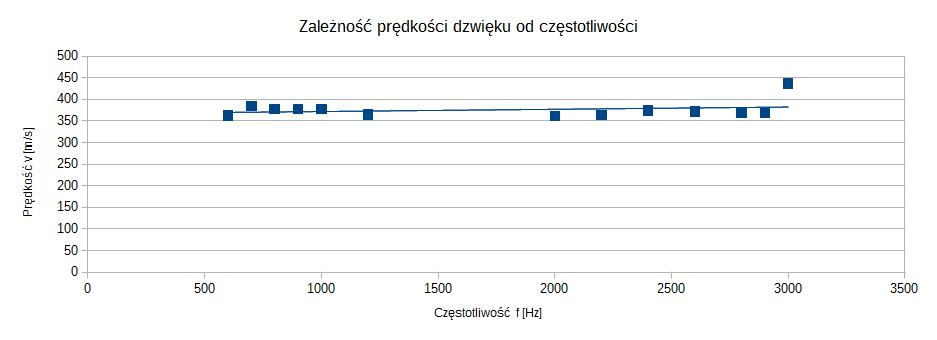
\includegraphics[scale=0.5]{ch01}
	\caption{Wykres zaleznosci v(f)}
\end{figure}

Widzimy, że dla pomiaru przy najwyższej częstotliwości mamy doczynienia z błędem grubym.

\subsection{Obliczenie średniej wartości prędkości i niepewności standardowej typu A}
Odrzucając błąd gruby (wynikał on z przegapienia jednego minimum), otrzymujemy prędkość dźwięku v wynoszącą $3.7 \cdot 10^2$ $\frac{m}{s}$
Korzystając z funkcji w LibreOffice Calc otrzymujemy niepewność standardową prędkości na poziomie 7.3 $\frac{m}{s}$

\subsection{Obliczenie prędkości dźwięku w gazie przy temperaturze $0^{o} C$}
Korzystając z wyliczonej wartości i formuły:
\begin{equation}
	v = \sqrt{\frac{\kappa RT}{\mu}}
\end{equation}
Otrzymujemy v = $3.58 \cdot 10^2$ $\frac{m}{s}$

\subsection{Porównanie wartości obliczonej z rzeczywistością}
Niestety dopiero uwzględniając współczynnik k = 4, otrzymujemy wartość mieszczącą się w przedziale błędu $3.58 \cdot 10^2 \frac{m}{s} +/- 29.04 \frac{m}{s}$

\subsection{Obliczenie współczynnika adiabaty $\kappa$}

Korzystając z powyższego związku otrzymujemy:
\begin{equation}
	\kappa = \frac{v^{2}\mu}{RT}
\end{equation}

Uwzględniając masy molowe pierwiastków występujących w powietrzu i wyliczając średnią ważoną otrzymujemy $\mu = 28.97 \frac{g}{mol} = 2.9 \cdot 10^{-2} \frac{kg}{mol}$. Po podstawieniu otrzymujemy $\kappa$ równą 1.64, która odbiega od rzeczywistej wynoszącej 1.4 o 17\% i mieści się w obliczonej poniżej niepewności.

Liczymy niepewność złożoną $\kappa$:
\begin{equation}
	u(\kappa) = \sqrt{(\frac{2v\mu}{RT} \cdot u(v))^2 + (\frac{v^2\mu}{RT^2} \cdot u(T))^2} = \sqrt{(\frac{2 \cdot 358.2 \cdot 2.9 \cdot 10^{-2}}{8.31 \cdot 294} \cdot 29.04)^2+(\frac{(358.2)^2 \cdot 2.9 \cdot 10^{-2}}{8.31 \cdot (294)^2} \cdot 1)^2}
\end{equation}
\begin{equation}
	u(\kappa) = \sqrt{0.06098+2.68 \cdot 10^{-5}} \approx 0.25
\end{equation}
%----------------------------------------------------------------------------------------
%	SECTION 6
%----------------------------------------------------------------------------------------
\section{Wnioski}

Doswiadczenie wykazało poprawność metody wyznaczania prędkości dźwięku w gazach przy pomocy wykorzystania zjawiska interferencji falowej.
Uwględniając niepewność rozszerzoną k = 4 uzyskaliśmy wynik zgodny z wartością tabelaryczną dla powietrza w temperaturze 273 K;
tabelaryczna = \textbf{$3.3 \cdot 10^{2}$ $\frac{m}{s}$} uzyskana w doświadczeniu = \textbf{\textbf{$3.58 \cdot 10^2$} $\frac{m}{s}$}. 
\\
Wartość $\kappa$ przy wykorzystaniu tej samej niepewności rozszerzonej wyniosła \textbf{1.64}, w porównaniu do tabelarycznej \textbf{(1.4)}.


%----------------------------------------------------------------------------------------
%	BIBLIOGRAPHY
%----------------------------------------------------------------------------------------

\bibliographystyle{apalike}

\bibliography{sample}
%----------------------------------------------------------------------------------------


\end{document}
